% Author: Izaak Neutelings (August 2021)
% Sources & inspiration:
%  Physics from Symmetry (Jakob Schwichtenberg)
%  https://doi.org/10.3390/sym8090087 (Andreas Aste, https://www.mdpi.com/2073-8994/8/9/87/htm)
%  https://arxiv.org/abs/1705.02227 (V.V. Varlamov)
%  https://en.wikiversity.org/wiki/Representation_theory_of_the_Lorentz_group
\documentclass[border=2pt,tikz]{standalone}
\usepackage{tikz}
\usepackage{amsmath} % for \dfrac, \text, aligned
\usepackage{amssymb} % for \mathfrak
\usepackage{bbold} % for \mathbb
\usepackage[outline]{contour} % glow around text
\usetikzlibrary{arrows.meta} % to control arrow size
\usepackage{xcolor} % for colored text
\tikzset{>=latex} % for LaTeX arrow head
\contourlength{1.2pt}

\newcommand\LP{{\color{mydarkblue}P}} %\Lambda_\mathrm{P}
\newcommand\LT{{\color{mydarkred}T}} %\Lambda_\mathrm{T}
\colorlet{myred}{red!60!black}
\colorlet{myblue}{blue!60!black}
\colorlet{mygreen}{green!60!black}
\colorlet{mydarkblue}{blue!40!black}
\colorlet{mydarkred}{red!40!black}
\colorlet{mydarkgreen}{green!40!black}
\colorlet{mydarkpurple}{blue!50!red!50!black}
\tikzstyle{myarr}=[-{Latex[length=4,width=3]}]

\begin{document}


% LORENTZ TRANSFORMATIONS
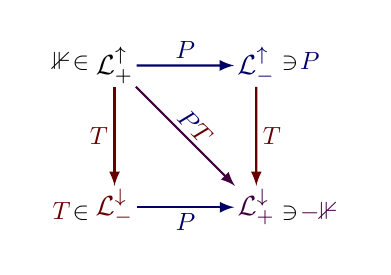
\begin{tikzpicture}[scale=1.8]
  \def\is{1.0} % inner seperation of nodes
  
  % GROUPS
  \node[inner sep=\is,mydarkred] (Ld-) at (0,0) {$\mathcal{L}^\downarrow_-$};
  \node[inner sep=\is] (Lu+) at (0,1) {$\mathcal{L}^\uparrow_+$}; % SO+(1,3)
  \node[inner sep=\is,mydarkblue] (Lu-) at (1,1) {$\mathcal{L}^\uparrow_-$};
  \node[inner sep=\is,mydarkpurple] (Ld+) at (1,0) {$\mathcal{L}^\downarrow_+$};
  
  % ELEMENTS
  \node[anchor=-5,inner sep=10,scale=0.9] at (Lu+) {$\mathbb{1}\hspace{-.2em}\in$};
  \node[anchor= 5,inner sep=10,scale=0.9] at (Ld-) {$\LT\hspace{-.2em}\in$};
  \node[anchor=185,inner sep=10,scale=0.9] at (Lu-) {$\ni\hspace{-.2em}\LP$};
  \node[anchor=175,inner sep=10,scale=0.9] at (Ld+) {$\ni\hspace{-.2em}\color{mydarkpurple}-\mathbb{1}$};
  
  % ARROWS
  \draw[->,thick,mydarkred] (Lu+) -- (Ld-)
    node[midway,left=-1,scale=0.9] {$\LT$};
  \draw[->,thick,mydarkblue] (Lu+) -- (Lu-)
    node[midway,above=-1,scale=0.9] {$\LP$};
  \draw[->,thick,mydarkred] (Lu-) -- (Ld+)
    node[midway,right=-1,scale=0.9] {$\LT$};
  \draw[->,thick,mydarkblue] (Ld-) -- (Ld+)
    node[midway,below=-1,scale=0.9] {$\LP$};
  \draw[->,thick,mydarkpurple] (Lu+) -- (Ld+)
    node[pos=0.3,above right=-1,scale=0.9,rotate=-45]
      {$\LP\LT$};
  
\end{tikzpicture}


% LORENTZ TRANSFORMATIONS
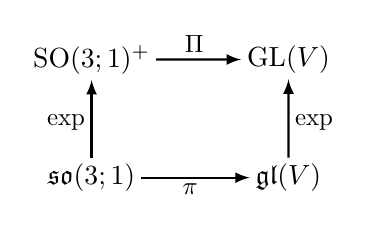
\begin{tikzpicture}[xscale=2.5,yscale=1.5]
  \def\is{2.0} % inner seperation of nodes
  
  % GROUPS
  \node[inner sep=\is] (so) at (0,0) {$\mathfrak{so}(3;1)$};
  \node[inner sep=\is] (SO) at (0,1) {$\mathrm{SO}(3;1)^+$};
  \node[inner sep=\is] (GL) at (1,1) {$\mathrm{GL}(V)$};
  \node[inner sep=\is] (gl) at (1,0) {$\mathfrak{gl}(V)$};
  
  % ARROWS
  \draw[->,thick] (so) -- (SO) node[pos=0.45,left=-1,scale=0.9] {$\exp$};
  \draw[->,thick] (gl) -- (GL) node[pos=0.45,right=-1,scale=0.9] {$\exp$};
  \draw[->,thick] (SO) -- (GL) node[pos=0.45,above=-1,scale=0.9] {$\Pi$};
  \draw[->,thick] (so) -- (gl) node[pos=0.45,below=-1,scale=0.9] {$\pi$};
  
\end{tikzpicture}


% LORENTZ GROUP (DOUBLE COVER) REPRESENTATIONS
% Inspired by https://arxiv.org/abs/1705.02227 (V.V. Varlamov)
% https://en.wikiversity.org/wiki/Representation_theory_of_the_Lorentz_group#Common_representations
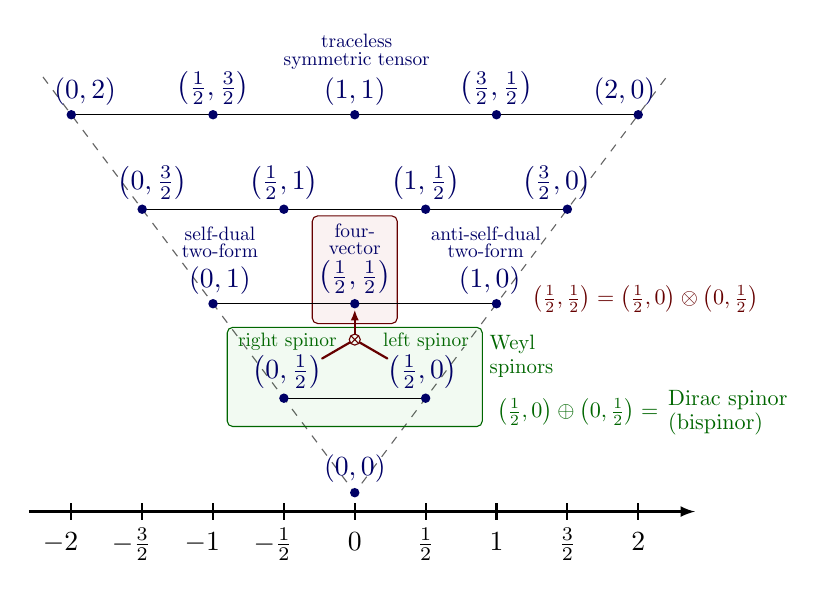
\begin{tikzpicture}[x=1.8cm,y=1.2cm]
  \def\N{4}      % number of spin states
  \def\r{0.07cm} % radius otimes
  \def\repr#1{   % format simple fraction
    \pgfmathsetmacro{\double}{int(2*#1)}
    \pgfmathsetmacro{\sign}{ifthenelse(#1<0,"-","")}
    \pgfmathparse{int(mod(\double,2))}
    \ifnum0=\pgfmathresult\relax % even
      \pgfmathprintnumber{#1}
    \else % odd
      \sign % sign
      \pgfmathparse{abs(int(\double))}
      \frac{\pgfmathprintnumber{\pgfmathresult}}{2}
    \fi
    \phantom{\sign} % for centered alignment
  }
  
  % AXIS
  \begin{scope}[shift={(0,-0.2)}]
    \draw[->,thick] (-\N/2-0.3,0) -- (\N/2+0.4,0); %node[right=-1] {$S$};
    \foreach \j [evaluate={\x=\j/2; \m=\j/2;}] in {-\N,...,\N}{ % ticks
      \draw[thick] (\x,0.09) --++ (0,-0.18)
        node[below=-1] {\strut$\repr{\m}$}; 
    }
  \end{scope}
  
  % LABELS Dirac spinor
  \draw[dashed,opacity=0.6] (-1.1*\N/2,1.1*\N) -- (0,0) -- (1.1*\N/2,1.1*\N);
  \draw[mydarkgreen,fill=mygreen,fill opacity=0.05,rounded corners=2]
    (-0.9,0.7) rectangle (0.9,1.75)
    node[mydarkgreen,below right,align=left,opacity=1,scale=0.75] {Weyl\\spinors};
  \node[mydarkgreen,scale=0.8,below right] at (0.95,1.2)
    {$\left(\frac{1}{2},0\right)\oplus\left(0,\frac{1}{2}\right)
       = \!\! \begin{array}{l}
           \text{Dirac spinor}\\[-0.5mm]
           \text{(bispinor)}
         \end{array}$};
  %\node[mydarkgreen,scale=0.8,below,align=center] at (1.55,0.68)
  %  {Dirac spinor\\[-3](bispinor)};
  %\node[mydarkgreen,scale=0.8,below,align=center] at (2.58,0.68)
  %  {four-\\[-3]vector};
  %\node[mydarkgreen,scale=0.8,below right] at (1.5,2.2)
  %  {$(1,0)\oplus(0,1) = \text{adjoint}$}; % parity-invariant 2-form field
  
  % LABELS four-vector
  \draw[mydarkred,fill=myred,fill opacity=0.05,rounded corners=2]
    (-0.3,1.79) rectangle (0.3,2.93);
  \node[mydarkred,scale=0.8,right] at (1.2,2.05)
    {$\left(\frac{1}{2},\frac{1}{2}\right) = %\cong
      \left(\frac{1}{2},0\right)\otimes\left(0,\frac{1}{2}\right)$};
  
  % DOTS
  \foreach \j [evaluate={\y=\j;}] in {0,...,\N}{
    \draw (-\j/2,\y) --++ (\j,0);
    \foreach \i [evaluate={
      \m=\i-\j/2;
      \L=\i/2; % left representation
      \R=\j/2-\i/2; % right representation
      \x=\m; % x position
      \myshift=((\i==0||\i==\j)?-2.5*\x:0);
    }] in {0,...,\j}{
      \fill[mydarkblue] (\x,\y) circle (0.06cm);
      \node[mydarkblue,right=\myshift,above]
        %,fill=white,text opacity=1,fill opacity=0.5,inner sep=0.5,outer sep=3
        (P\j-\i) at (\x,\y) {$\left(\repr{\L},\repr{\R}\right)$};
    }
  }
  
  % ARROWS & OTIMES
  \draw[thick,mydarkred,line cap=round]
    (-0.23,1.42) -- (0,1.62) coordinate (A) -- (0.23,1.42);
  \draw[myarr,thick,mydarkred,line cap=round]
    (A) -- (0,1.94);
  \draw[mydarkred,line width=0.4,fill=mygreen!5] % circle
    (A) circle(\r);
  \draw[mydarkred,line width=0.4] % cross
    (A)++(45:\r) --++ (-135:2*\r)
    (A)++(135:\r) --++ (-45:2*\r);
  
  % LABELS
  \node[mydarkgreen,scale=0.7,above=6]
    at (P1-0) {\strut\contour{mygreen!5}{right spinor}};
  \node[mydarkgreen,scale=0.7,right=2,above=6]
    at (P1-1) {\strut\contour{mygreen!5}{left spinor}};
  \node[mydarkblue,scale=0.7,above=8,align=center]
    at (P2-0) {self-dual\\[-3]two-form};
  \node[mydarkblue,scale=0.7,above=8,align=center]
    at (P2-1) {four-\\[-3]vector};
  \node[mydarkblue,scale=0.7,left=2,above=8,align=center]
    at (P2-2) {anti-self-dual\\[-3]two-form};
  \node[mydarkblue,scale=0.7,right=1,above=8,align=center]
    at (P4-2) {traceless\\[-3]symmetric tensor};
  
\end{tikzpicture}


\end{document}
